\documentclass[11pt]{article}
\usepackage{xcolor}
\usepackage[utf8]{inputenc}
\usepackage[english]{babel}
\usepackage{fullpage}
\usepackage{graphicx}

\begin{document}
\pagecolor{gray}
\begin{Huge}
\title{\color{green}\textit{\Huge\bfseries Cloud Computing }\line(1,0){210}}
\author{\color{black} md.zakir Hossen\\
Id:18ictcse057}
\date{\color{black} \today}
\end{Huge}
\maketitle
\begin{figure}
\begin{center}


\includegraphics[scale=.2]{a1.jpg}
\begin{center}
Bangabandhu Sheikh Mujibur Rahaman Science  Technology University

Gopalgonj.
 \end{center}
\end{center}
\end{figure}
\newpage
\bfseries{\color{cyan}Cloud computing} smallis the on-demand availability of computer system resources, especially data storage and computing power, without direct active management by the user. The term is generally used to describe data centers available to many users over the Internet. Large clouds, predominant today, often have functions distributed over multiple locations from central servers. If the connection to the user is relatively close, it may be designated an edge server.
Clouds may be limited to a single organization (enterprise clouds[1][2]), or be available to many organizations (public cloud).
Cloud computing relies on sharing of resources to achieve coherence and economies of scale.
Advocates of public and hybrid clouds note that cloud computing allows companies to avoid or minimize up-front IT infrastructure costs. Proponents also claim that cloud computing allows enterprises to get their applications up and running faster, with improved manageability and less maintenance, and that it enables IT teams to more rapidly adjust resources to meet fluctuating and unpredictable demand,[2][3][4] providing the burst computing capability: high computing power at certain periods of peak demand.[5] operating expenses if administrators are not familiarized with cloud-pricing models.
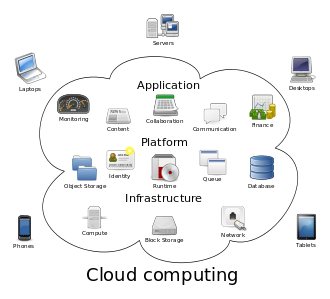
\includegraphics[scale=1]{a4.png}
\newpage
\tableofcontents
\newpage
\section{\color{green}History}
Cloud computing was popularized with Amazon.com releasing its Elastic Compute Cloud product in 2006.[12]

References to the phrase "cloud computing" appeared as early as 1996, with the first known mention in a Compaq internal document.[13]

The cloud symbol was used to represent networks of computing equipment in the original ARPANET by as early as 1977,[14] and the CSNET by 1981[15]—both predecessors to the Internet itself.
\section{\color{green}Characteristics}
\begin{itemize}
\item Agility for organizations may be improved, as cloud computing may increase users' flexibility with re-provisioning, adding, or expanding technological infrastructure resources.
\item Cost reductions are claimed by cloud providers. A public-cloud delivery model converts capital expenditures (e.g., buying servers) to operational expenditure.
\item \textcolor{blue}{Device and location} independence[49] enable users to access systems using a web browser regardless of their location or what device they use (e.g., PC, mobile phone).
\item \textcolor{blue}{Maintenance} of cloud computing applications is easier, because they do not need to be installed on each user's computer and can be accessed from different places (e.g., different work locations, while travelling, etc.).
\item \textcolor{blue}{Multitenancy}enables sharing of resources and costs across a large pool of users thus allowing for:
\begin{itemize}
\item centralization of infrastructure in locations with lower costs (such as real estate, electricity, etc.)
\item  peak-load capacity increases (users need not engineer and pay for the resources and equipment to meet their highest possible load-levels)
\item utilisation and efficiency improvements for systems that are often only
 10–20.
\end{itemize}
\end{itemize}
\section{\color{green}Service models}
Though service-oriented architecture advocates "Everything as a service" (with the acronyms EaaS or XaaS,[64] or simply aas), cloud-computing providers offer their "services" according to different models, of which the three standard models per NIST are Infrastructure as a Service (IaaS), Platform as a Service (PaaS), and Software as a Service (SaaS).
\begin{center}

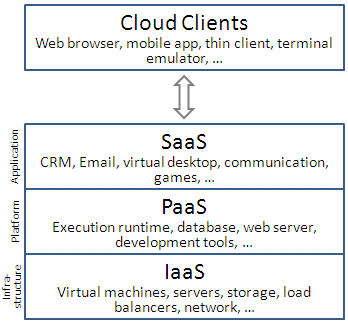
\includegraphics[scale=0.5]{a2.png} 
\end{center}
These models offer increasing abstraction; they are thus often portrayed as a layers in a stack: infrastructure-, platform- and software-as-a-service, but these need not be related. 
\subsection{\textcolor{magenta}{Infrastructure as a service (IaaS)}}
"Infrastructure as a service" (IaaS) refers to online services that provide high-level APIs used to dereference various low-level details of underlying network infrastructure like physical computing resources, location, data partitioning, scaling, security, backup etc. A hypervisor runs the virtual machines as guests. Pools of hypervisors within the cloud operational system can support large numbers of virtual machines and the ability to scale services up and down according to customers' varying requirements. Linux containers run in isolated partitions of a single Linux kernel running directly on the physical hardware.
\subsection{\textcolor{magenta}{Platform as a service (PaaS)}}
The capability provided to the consumer is to deploy onto the cloud infrastructure consumer-created or acquired applications created using programming languages, libraries, services, and tools supported by the provider. The consumer does not manage or control the underlying cloud infrastructure including network, servers, operating systems, or storage, but has control over the deployed applications and possibly configuration settings for the application-hosting environment.
\subsection{\textcolor{magenta}{Software as a service (SaaS)}}
The capability provided to the consumer is to use the provider's applications running on a cloud infrastructure. The applications are accessible from various client devices through either a thin client interface, such as a web browser (e.g., web-based email), or a program interface.
\subsection{\textcolor{magenta}{Serverless computing}}
Serverless computing is a cloud computing code execution model in which the cloud provider fully manages starting and stopping virtual machines as necessary to serve requests, and requests are billed by an abstract measure of the resources required to satisfy the request, rather than per virtual machine, per hour.[82] Despite the name, it does not actually involve running code without servers.
\section{\color{green}{Deployment models}}
\subsection{\textcolor{magenta}{Private Cloud}}
Private cloud is cloud infrastructure operated solely for a single organization, whether managed internally or by a third party, and hosted either internally or externally
\subsection{\textcolor{magenta}{Public Cloud}}
A cloud is called a "public cloud" when the services are rendered over a network that is open for public use. Public cloud services may be free.[89] Technically there may be little or no difference between public and private cloud architecture, however, security consideration may be substantially different for services (applications, storage, and other resources) that are made available by a service provider for a public audience and when communication is effected over a non-trusted network
\subsection{\textcolor{magenta}{Hybrid Cloud}}
Hybrid cloud is a composition of a public cloud and a private environment, such as a private cloud or on-premise resources,[91][92][93] that remain distinct entities but are bound together, offering the benefits of multiple deployment models. Hybrid cloud can also mean the ability to connect collocation, managed and/or dedicated services with cloud resources.[63] Gartner defines a hybrid cloud service as a cloud computing service that is composed of some combination of private, public and community cloud services, from different service providers.
\subsection{\textcolor{magenta}{Other}}
\subsubsection{\textcolor{yellow}{Community cloud}}
Community cloud shares infrastructure between several organizations from a specific community with common concerns (security, compliance, jurisdiction, etc.), whether managed internally or by a third-party, and either hosted internally or externally. 
\subsubsection{\textcolor{yellow}{Distributed  cloud}}
A cloud computing platform can be assembled from a distributed set of machines in different locations, connected to a single network or hub service. It is possible to distinguish between two types of distributed clouds: public-resource computing and volunteer cloud.
\begin{itemize}
\item \textbf{Public-resource computing—}\texttt{
This type of distributed cloud results from an expansive definition of cloud computing, because they are more akin to distributed computing than cloud computing. Nonetheless, it is considered a sub-class of cloud computing.}
\item \textbf{Volunteer cloud—}\texttt{Volunteer cloud computing is characterized as the intersection of public-resource computing and cloud computing, where a cloud computing infrastructure is built using volunteered resources. Many challenges arise from this type of infrastructure, because of the volatility of the resources used to built it and the dynamic environment it operates in.}

\end{itemize}
\subsubsection{\textcolor{yellow}{Multicloud}}
Multicloud is the use of multiple cloud computing services in a single heterogeneous architecture to reduce reliance on single vendors, increase flexibility through choice, mitigate against disasters, etc. It differs from hybrid cloud in that it refers to multiple cloud services, rather than multiple deployment modes (public, private, legacy)
\subsubsection{\textcolor{yellow}{Poly cloud}}
Poly cloud refers to the use of multiple public clouds for the purpose of leveraging specific services that each provider offers. It differs from multicloud in that it is not designed to increase flexibility or mitigate against failures but is rather used to allow an organisation to achieve more that could be done with a single provide
\subsubsection{\textcolor{yellow}{Big Data cloud}}
The issues of transferring large amounts of data to the cloud as well as data security once the data is in the cloud initially hampered adoption of cloud for big data, but now that much data originates in the cloud and with the advent of bare-metal servers, the cloud has become[107] a solution for use cases including business analytics and geospatial analysis
\section{\color{green}Architecture}
\textcolor{blue}{Cloud architecture} the systems architecture of the software systems involved in the delivery of cloud computing, typically involves multiple cloud components communicating with each other over a loose coupling mechanism such as a messaging queue.\\ Elastic provision implies intelligence in the use of tight or loose coupling as applied to mechanisms such as these and others.\\
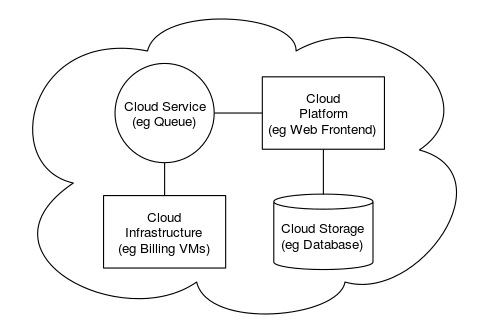
\includegraphics[scale=.4]{a3.png}
\subsection{\textcolor{magenta}{Cloud engineering}}
\textcolor{blue}{Cloud engineering} is the application of engineering disciplines to cloud computing. It brings a systematic approach to the high-level concerns of commercialization, standardization, and governance in conceiving, developing, operating and maintaining cloud computing systems. It is a multidisciplinary method encompassing contributions from diverse areas such as systems, software, web, performance, information technology engineering, security, platform, risk, and quality engineering.
\section{\color{green}Security and privacy}
Cloud computing poses privacy concerns because the service provider can access the data that is in the cloud at any time. It could accidentally or deliberately alter or delete information.[115] Many cloud providers can share information with third parties if necessary for purposes of law and order without a warrant. That is permitted in their privacy policies, which users must agree to before they start using cloud services. Solutions to privacy include policy and legislation as well as end users' choices for how data is stored.[115] Users can encrypt data that is processed or stored within the cloud to prevent unauthorized access\textit{Insecure Interfaces and API's, Data Loss and Leakage, and Hardware Failure—}
\section{\color{green}Limitations and disadvantages}
According to \textcolor{red}{Bruce Schneier}, "The downside is that you will have limited customization options. Cloud computing is cheaper because of economics of scale, and—like any outsourced task—you tend to get what you want. A restaurant with a limited menu is cheaper than a personal chef who can cook anything you want. Fewer options at a much cheaper price: it's a feature, not a bug." He also suggests that "the cloud provider might not meet your legal needs" and that businesses need to weigh the benefits of cloud computing against the risks.[121] In cloud computing, the control of the back end infrastructure is limited to the cloud vendor only. Cloud providers often decide on the management policies, which moderates what the cloud users are able to do with their deployment.[122] Cloud users are also limited to the control and management of their applications, data and services.[123] This includes data caps, which are placed on cloud users by the cloud vendor allocating certain amount of bandwidth for each customer and are often shared among other cloud users.
\section{\color{green}Emerging trends}Cloud computing is still a subject of research.[125] A driving factor in the evolution of cloud computing has been chief technology officers seeking to minimize risk of internal outages and mitigate the complexity of housing network and computing hardware in-house.[126] Major cloud technology companies invest billions of dollars per year in cloud Research and Development.
\section{\color{green}Digital forensics in the cloud}
The issue of carrying out investigations where the cloud storage devices cannot be physically accessed has generated a number of changes to the way that digital evidence is located and collected.[129] New process models have been developed to formalize collection.[130]

In some scenarios existing digital forensics tools can be employed to access cloud storage as networked drives (although this is a slow process generating a large amount of internet traffic).

\end{document}